\section{Appendix}
\label{sec:appendix}

\FloatBarrier

\subsection{Learned-Policy Comparison and GoalBuffer Recovery}

This subsection receives the learned-policy comparison block referenced from the main text. Table~\ref{tab:sac_baselines} together with Figures~\ref{fig:three_way}--\ref{fig:goalbuffer} compare learned and explicit memory, and we keep this evidence block here so that Table~\ref{tab:sac_baselines} stays in the appendix rather than drifting toward the conclusion.

\begin{table}[t]
\centering
\caption{Learned-policy comparison under FO, WeakPO, and StrongPO. SAC-MLP is trained under FO for 2M steps; SAC-LSTM under WeakPO for 2M steps. Entries are success rates (\%), reported as mean $\pm$ std over 3 seeds $\times$ 60 episodes unless marked $^\dagger$ (single seed). WeakPO masks goal position; StrongPO also masks object position (\texttt{flash\_every}$=$5, \texttt{flash\_len}$=$1).}
\label{tab:sac_baselines}
\begin{tabular}{l ccc}
\toprule
Task & Condition & SAC-MLP (FO-train) & SAC-LSTM (PO-train) \\
\midrule
\multirow{3}{*}{Reach-v3}
 & FO        & 78.9$\pm$6.0  & 47.8$\pm$9.0  \\
 & WeakPO    &  0.0$\pm$0.0  & 42.2$\pm$5.9  \\
 & StrongPO  &  0.0$\pm$0.0  & 29.4$\pm$6.5  \\
\midrule
\multirow{3}{*}{Faucet-Open-v3}
 & FO        & 100.0$\pm$0.0 & 74.4$\pm$35.6 \\
 & WeakPO    &   1.1$\pm$1.9 & 72.8$\pm$41.4 \\
 & StrongPO  &   5.0$\pm$8.7 &   1.1$\pm$1.9 \\
\midrule
\multirow{3}{*}{Door-Open-v3$^\dagger$}
 & FO        & 100.0 (n=1)   & ---            \\
 & WeakPO    &   0.0 (n=1)   & ---            \\
 & StrongPO  &   0.0 (n=1)   & ---            \\
\midrule
\multirow{3}{*}{Drawer-Open-v3$^\dagger$}
 & FO        & 100.0 (n=1)   & ---            \\
 & WeakPO    &  20.0 (n=1)   & ---            \\
 & StrongPO  &   0.0 (n=1)   & ---            \\
\bottomrule
\end{tabular}
\begin{flushleft}
\footnotesize SAC-MLP collapses under PO on all four tasks. SAC-LSTM shows high variance on Faucet-Open-v3 and trades FO performance for partial PO robustness on Reach-v3. GoalBuffer recovers WeakPO to 82--100\% without retraining (Table~\ref{tab:goal_buffer}). $^\dagger$ denotes single-seed SAC-MLP results; Pick-Place/Push/Button-Press are excluded because FO learning does not become reliable within 2M steps.
\end{flushleft}
\end{table}

\begin{figure}[t]
\centering
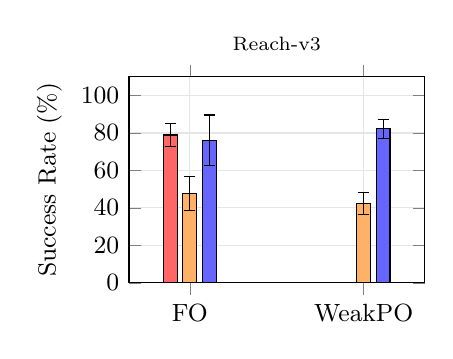
\begin{tikzpicture}
\begin{axis}[
    ybar,
    width=0.44\textwidth,
    height=4.2cm,
    bar width=5pt,
    ymin=0, ymax=110,
    ytick={0,20,40,60,80,100},
    symbolic x coords={FO, WeakPO},
    xtick=data,
    enlarge x limits=0.35,
    grid=major,
    grid style={gray!20},
    ylabel={Success Rate (\%)},
    error bars/y dir=both,
    error bars/y explicit,
    tick label style={font=\small},
    label style={font=\small},
    title={\scriptsize Reach-v3},
]
\addplot[fill=red!60] coordinates {(FO,78.9) +- (0,6.0) (WeakPO,0.0) +- (0,0.0)};
\addplot[fill=orange!60] coordinates {(FO,47.8) +- (0,9.0) (WeakPO,42.2) +- (0,5.9)};
\addplot[fill=blue!60] coordinates {(FO,76.1) +- (0,13.5) (WeakPO,82.2) +- (0,5.0)};
\end{axis}
\end{tikzpicture}
\hfill
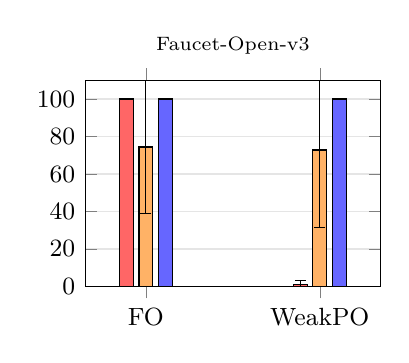
\begin{tikzpicture}
\begin{axis}[
    ybar,
    width=0.44\textwidth,
    height=4.2cm,
    bar width=5pt,
    ymin=0, ymax=110,
    ytick={0,20,40,60,80,100},
    symbolic x coords={FO, WeakPO},
    xtick=data,
    enlarge x limits=0.35,
    grid=major,
    grid style={gray!20},
    error bars/y dir=both,
    error bars/y explicit,
    tick label style={font=\small},
    title={\scriptsize Faucet-Open-v3},
]
\addplot[fill=red!60] coordinates {(FO,100.0) +- (0,0.0) (WeakPO,1.1) +- (0,1.9)};
\addplot[fill=orange!60] coordinates {(FO,74.4) +- (0,35.6) (WeakPO,72.8) +- (0,41.4)};
\addplot[fill=blue!60] coordinates {(FO,100.0) +- (0,0.0) (WeakPO,100.0) +- (0,0.0)};
\end{axis}
\end{tikzpicture}
\par\vspace{1mm}
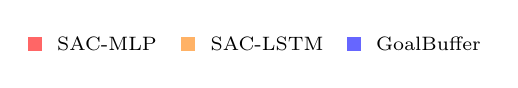
\begin{tikzpicture}[baseline]
\fill[red!60] (0,0) rectangle (0.18,0.18);
\node[anchor=west, font=\scriptsize] at (0.25,0.09) {SAC-MLP};

\fill[orange!60] (1.95,0) rectangle (2.13,0.18);
\node[anchor=west, font=\scriptsize] at (2.20,0.09) {SAC-LSTM};

\fill[blue!60] (4.05,0) rectangle (4.23,0.18);
\node[anchor=west, font=\scriptsize] at (4.30,0.09) {GoalBuffer};
\end{tikzpicture}
\caption{Three-way comparison on Reach-v3 and Faucet-Open-v3. Bars show mean over 3 seeds $\times$ 60 episodes; error bars denote std. SAC-LSTM is high-variance on Faucet-Open-v3 ($\sigma=41.4\%$), while GoalBuffer recovers WeakPO to 82.2--100\% on both tasks.}
\label{fig:three_way}
\end{figure}

\input{figures/fig_goalbuffer}

\FloatBarrier

\input{figures/fig_flash_every}

\subsection{Task Details}

All 9 tasks use the MuJoCo \citep{Todorov2012} simulator via MetaWorld V3 \citep{Yu2020} with 200-step episodes. Observation dimensions range from 10 (Reach-v3) to 23 (Pick-Place-v3); action dimension is 4 for all tasks. Rule-based experiments use fixed seeds $\{0,1,2,3,4\}$; learned policies and Gymnasium-Robotics use $\{0,1,2\}$.

\subsection{PO Wrapper Implementation}

The PO wrapper operates on the observation vector: on non-flash steps, it zeros out the goal position (WeakPO) or both goal and object positions (StrongPO). The flash schedule is deterministic: the goal is revealed for \texttt{flash\_len} steps every \texttt{flash\_every} steps, starting from step 0.

\subsection{SAC Hyperparameters}

\begin{itemize}
\item Learning rate: 3e-4 (actor and critic)
\item Discount factor $\gamma$: 0.99
\item Soft update coefficient $\tau$: 0.005
\item Replay buffer size: 1,000,000
\item Batch size: 256
\item Training starts at step 10,000
\item MLP: 2 hidden layers of 256 units with ReLU
\item LSTM: 128 hidden units, unroll length 20
\end{itemize}

\subsection{GoalBuffer Implementation}

See \S\ref{sec:experimental-setup} for the GoalBuffer definition. Under StrongPO, the object position remains masked (not cached), which is why GoalBuffer only partially recovers StrongPO performance.

\subsection{Push-v3 Variance Analysis}

Push-v3 shows high variance across seeds under FO (mean 64.3\%, std 29.7\%). This is because the task is near the boundary of open-loop solvability: some seeds place the arm close enough to the goal that the push succeeds regardless of observation, while others require precise goal-relative positioning. This variance is not an artifact of our framework but reflects the task's moderate goal-dependency ($G = 0.64$).

\subsection{StrongPO Full Results}

Under StrongPO, all 9 tasks $\times$ 3 rule-based policy variants yield 0.0$\pm$0.0\% success rate (5 seeds $\times$ 60 episodes). The complete results are visualized in Figure~\ref{fig:goal_dependency}.

\subsection{Door-Open-v3 Learned-Policy Single-Seed Limitation}

This subsection refers to the SAC-MLP learned-policy result in Table~\ref{tab:sac_baselines}. Door-Open-v3 seed 0 achieves 100\% under FO but 0\% under both WeakPO and StrongPO. Seeds 1--2 were not completed within the training budget. We present seed 0 as a single-seed limitation case for the learned SAC-MLP baseline: under this trained policy and masking protocol, sustained contact with a partially observed mechanism is not recovered without an explicit goal buffer or additional state estimation.

Drawer-Open-v3 (seed 0, single seed) achieves FO 100.0 / WeakPO 20.0 / StrongPO 0.0. The non-zero WeakPO result likely reflects that the initial drawer configuration provides partial goal information through object state before the goal is masked.

\subsection{Full Flash-Every Ablation Results}

Figure~\ref{fig:flash_every} above visualizes the flash-every ablation for Reach-v3 and Door-Open-v3. Table~\ref{tab:flash_every} provides the full numerical results for these two tasks across all flash frequencies. Table~\ref{tab:flash_every_full} reports the remaining tasks. This ablation was run as an independent 5-seed batch from Table~\ref{tab:main_results}; therefore the \texttt{flash\_every}$=20$ rows can differ slightly from the main-table PO numbers. The pattern is consistent: NoMemory degrades monotonically with increasing flash interval, while TextBuffer and StructMemory remain near-FO performance across all flash frequencies.

\begin{table}[t]
\centering
\caption{Success rates (\%) under varying goal flash frequency (\texttt{flash\_every}). Mean $\pm$ std over 5 seeds $\times$ 60 episodes. At \texttt{flash\_every}$=k$, the goal is visible for 1 step every $k$ steps; $k$=1 means goal visible every step (FO equivalent).}
\label{tab:flash_every}
\begin{tabular}{l ccc}
\toprule
flash\_every & NoMemory & TextBuffer & StructMemory \\
\midrule
\multicolumn{4}{l}{\textit{Reach-v3}} \\
1  & 82.3$\pm$9.5 & 82.3$\pm$9.5 & 82.3$\pm$9.5 \\
5  & 38.7$\pm$9.5 & 75.0$\pm$6.4 & 75.0$\pm$6.4 \\
10 & 4.0$\pm$8.0 & 73.7$\pm$9.5 & 73.7$\pm$9.5 \\
20 & 0.0$\pm$0.0 & 69.7$\pm$6.1 & 69.7$\pm$6.1 \\
50 & 0.0$\pm$0.0 & 60.0$\pm$7.1 & 60.0$\pm$7.1 \\
\midrule
\multicolumn{4}{l}{\textit{Door-Open-v3}} \\
1  & 90.3$\pm$5.7 & 91.0$\pm$5.1 & 90.3$\pm$5.7 \\
5  & 0.0$\pm$0.0 & 91.0$\pm$5.1 & 90.7$\pm$5.2 \\
10 & 0.0$\pm$0.0 & 90.7$\pm$5.6 & 91.0$\pm$4.8 \\
20 & 0.0$\pm$0.0 & 90.7$\pm$5.6 & 90.7$\pm$5.2 \\
50 & 0.0$\pm$0.0 & 91.0$\pm$5.1 & 91.0$\pm$4.8 \\
\bottomrule
\end{tabular}
\end{table}

\begin{table}[t]
\centering
\caption{Success rates (\%) under WeakPO with varying \texttt{flash\_every} for Push-v3, Pick-Place-v3, and Sweep-v3. Mean $\pm$ std over 5 seeds $\times$ 60 episodes. Caveat: this table comes from the independent flash-frequency ablation batch described above, so the \texttt{flash\_every}$=20$ rows can differ slightly from Table~\ref{tab:main_results}; the FO-equivalent \texttt{flash\_every}$=1$ case is omitted because it is already reported in Table~\ref{tab:flash_every}.}
\label{tab:flash_every_full}
\begin{tabular}{l cccc}
\toprule
Task & flash\_every & NoMemory & TextBuffer & StructMemory \\
\midrule
\multirow{4}{*}{Push-v3}
 & 5  & 41.7$\pm$39.1 & 66.3$\pm$23.9 & 64.3$\pm$24.7 \\
 & 10 & 10.7$\pm$7.2  & 66.7$\pm$23.3 & 64.7$\pm$24.7 \\
 & 20 &  0.0$\pm$0.0  & 66.7$\pm$25.1 & 64.7$\pm$26.1 \\
 & 50 &  0.0$\pm$0.0  & 67.3$\pm$26.0 & 64.0$\pm$27.5 \\
\midrule
\multirow{4}{*}{Pick-Place-v3}
 & 5  &  0.0$\pm$0.0  & 75.0$\pm$5.1  & 75.0$\pm$5.1 \\
 & 10 &  0.0$\pm$0.0  & 73.7$\pm$6.5  & 73.7$\pm$6.5 \\
 & 20 &  0.0$\pm$0.0  & 73.7$\pm$7.6  & 73.7$\pm$7.6 \\
 & 50 &  0.0$\pm$0.0  & 74.0$\pm$3.6  & 74.0$\pm$3.6 \\
\midrule
\multirow{4}{*}{Sweep-v3}
 & 5  &  0.0$\pm$0.0  & 50.0$\pm$5.9  & 50.0$\pm$5.9 \\
 & 10 &  0.0$\pm$0.0  & 51.7$\pm$5.7  & 52.3$\pm$4.9 \\
 & 20 &  0.0$\pm$0.0  & 51.0$\pm$3.2  & 51.7$\pm$2.4 \\
 & 50 &  0.0$\pm$0.0  & 53.7$\pm$5.3  & 53.7$\pm$6.2 \\
\bottomrule
\end{tabular}
\end{table}

\subsection{GoalBuffer Full Results}

Figure~\ref{fig:goalbuffer} above visualizes the GoalBuffer recovery under WeakPO. Table~\ref{tab:goal_buffer} provides the complete numerical results including StrongPO conditions. The ``No Buffer'' columns come from the GoalBuffer evaluation run itself and may differ slightly from Table~\ref{tab:sac_baselines}, which reports the standalone SAC baseline evaluation.

\subsection{Sequential Multi-Goal Results}

Table~\ref{tab:multi_goal} reports the sequential multi-goal evaluation referenced from the main text. The qualitative conclusion is unchanged: once a goal can be cached, point memory remains sufficient after the mid-episode goal switch.

\begin{table}[t]
\centering
\caption{Sequential multi-goal evaluation under WeakPO (\texttt{flash\_every}$=20$, \texttt{flash\_len}$=1$). Entries are success rates (\%) reported as mean $\pm$ std over 5 seeds $\times$ 60 episodes. Caveat: the goal switches exactly once mid-episode after the first success, with a one-step flash of the new target, so this is a controlled two-goal stress test rather than a general continual-goal benchmark.}
\label{tab:multi_goal}
\begin{tabular}{l ccc}
\toprule
Task & NoMemory & TextBuffer & StructMemory \\
\midrule
Reach-v3 & 40.0$\pm$7.7 & 70.7$\pm$12.0 & 70.0$\pm$11.6 \\
Push-v3 & 41.7$\pm$44.5 & 64.7$\pm$27.7 & 63.3$\pm$28.9 \\
Pick-Place-v3 & 0.0$\pm$0.0 & 73.0$\pm$6.1 & 73.0$\pm$6.1 \\
\bottomrule
\end{tabular}
\end{table}


\begin{table}[t]
\centering
\caption{GoalBuffer evaluation under WeakPO and StrongPO: FO-trained SAC-MLP checkpoints (2M steps) are evaluated with and without a goal-caching buffer using \texttt{flash\_every}$=5$ and \texttt{flash\_len}$=1$. Entries are success rates (\%), reported as mean $\pm$ std over 3 seeds $\times$ 60 episodes unless marked $^\dagger$ (single seed). Caveat: on non-flash steps only the goal coordinates are restored, so under StrongPO the object-position information remains masked.}
\label{tab:goal_buffer}
\begin{tabular}{l ccc ccc}
\toprule
& \multicolumn{3}{c}{No Buffer} & \multicolumn{3}{c}{GoalBuffer} \\
\cmidrule(lr){2-4} \cmidrule(lr){5-7}
Task & FO & WeakPO & StrongPO & FO & WeakPO & StrongPO \\
\midrule
Reach-v3 & 78.9$\pm$6.0 & 0.0 & 0.0 & 76.1$\pm$13.5 & \textbf{82.2$\pm$5.0} & \textbf{69.4$\pm$20.8} \\
Door-Open-v3$^\dagger$ & 100.0 & 0.0 & 0.0 & 100.0 & \textbf{100.0} & 0.0 \\
Drawer-Open-v3$^\dagger$ & 100.0 & 18.3 & 0.0 & 100.0 & \textbf{100.0} & 0.0 \\
Faucet-Open-v3 & 100.0$\pm$0.0 & 0.0$\pm$0.0 & 4.4$\pm$7.7 & 100.0$\pm$0.0 & \textbf{100.0$\pm$0.0} & 0.6$\pm$1.0 \\
Pick-Place-v3$^\dagger$ & 85.0 & 1.7 & 0.0 & 88.3 & \textbf{86.7} & 0.0 \\
\bottomrule
\end{tabular}
\end{table}

\subsection{Cross-Platform Validation Details}

Table~\ref{tab:cross_platform} provides the full numerical results for the Gymnasium-Robotics cross-platform validation across two tasks.

\begin{table}[t]
\centering
\caption{Cross-platform validation on Gymnasium-Robotics under FO, WeakPO, and StrongPO. Entries are success rates (\%) for rule-based policies with the same FSM backbone and memory variants as Table~\ref{tab:main_results}, averaged over 3 seeds $\times$ 60 episodes. Caveat: FetchReach-v4 has no manipulable object state beyond the end-effector goal, so StrongPO is not applicable and is marked as --- .}
\label{tab:cross_platform}
\begin{tabular}{l ccc ccc}
\toprule
& \multicolumn{3}{c}{FetchReach-v4} & \multicolumn{3}{c}{FetchPush-v4} \\
\cmidrule(lr){2-4} \cmidrule(lr){5-7}
Memory & FO & WeakPO & StrongPO & FO & WeakPO & StrongPO \\
\midrule
NoMemory     & 100.0 & 15.6  & ---   & 29.4  & 5.6   & 4.4 \\
TextBuffer   & 100.0 & \textbf{100.0} & --- & 29.4  & \textbf{29.4} & 4.4 \\
StructMemory & 100.0 & \textbf{100.0} & --- & 29.4  & \textbf{29.4} & 4.4 \\
\bottomrule
\end{tabular}
\end{table}

\subsection{Retry Budget Ablation}

Table~\ref{tab:retry} shows the effect of StructMemory's retry mechanism on success rate. Retry=3 \emph{hurts} Pick-Place by 54.4pp for TextBuffer and 51.0pp for StructMemory because each retry consumes episode budget, leaving insufficient steps for the place phase. Push and Reach are unaffected as they do not involve grasp-retry cycles.

\begin{table}[t]
\centering
\caption{Success rates (\%) under two retry-budget conditions. \texttt{max\_retries}=3 allows up to 3 FSM-level retries upon grasp failure; \texttt{max\_retries}=0 disables retries. Entries are mean $\pm$ std over 5 seeds $\times$ 60 episodes. Caveat: Push and Reach are retained as no-effect controls, so the observed degradation is specific to the multi-phase Pick-Place task.}
\label{tab:retry}
\begin{tabular}{l ccc}
\toprule
Task & Policy & retry=0 & retry=3 \\
\midrule
Pick-Place & TextBuffer & 74.7$\pm$5.5 & 20.3$\pm$4.3 \\
Pick-Place & StructMemory & 74.7$\pm$5.5 & 23.7$\pm$3.2 \\
\midrule
Push & TextBuffer & 65.7$\pm$26.7 & 65.7$\pm$26.7 \\
Push & StructMemory & 64.3$\pm$28.0 & 64.3$\pm$28.0 \\
\midrule
Reach & TextBuffer & 64.7$\pm$7.8 & 64.7$\pm$7.8 \\
Reach & StructMemory & 64.7$\pm$7.8 & 64.7$\pm$7.8 \\
\bottomrule
\end{tabular}
\end{table}
